\section{Design}

\subsection{System Architecture Diagrams}

\subsubsection{Component-Level Architecture}

The Lab 6.1 system involves three physical components: the Arduino Mega 2560, a momentary push button wired to digital pin~7 with the internal pull-up enabled, and a current-limited LED driven from digital pin~8. The microcontroller exchanges diagnostic text with a host PC through UART0, which is exposed by the on-board USB-to-serial bridge. The structural diagram in \citeimg{fig:system_structural_diagram} shows the data flow: a press event travels from the button through the GPIO peripheral and the \texttt{Button} driver into the FSM, the FSM updates its state and forwards the new Moore output to the \texttt{Led} driver and to the STDIO log, and the host terminal displays the resulting transition.

\begin{figure}[H]
\centering
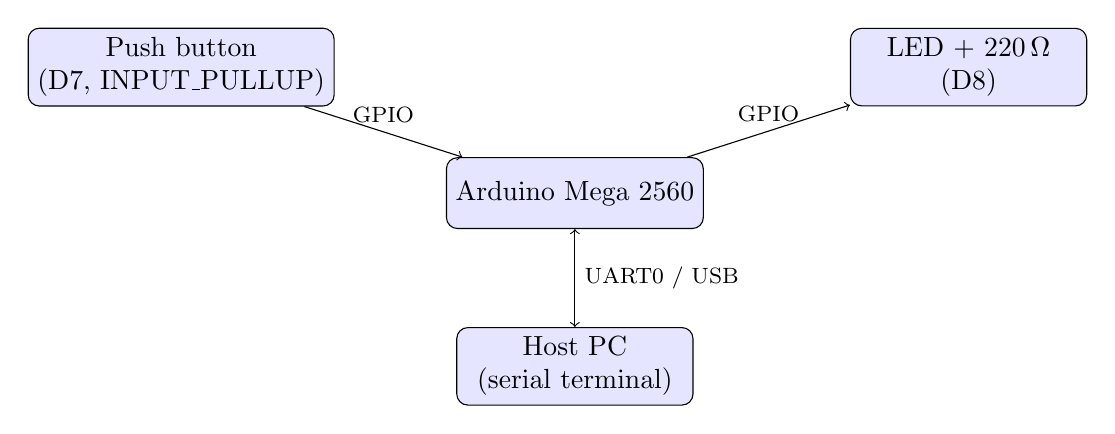
\begin{tikzpicture}[
    comp/.style={draw, rectangle, rounded corners, minimum width=3.0cm,
                 minimum height=0.9cm, text centered, align=center, fill=blue!10}]
    \node[comp] (mcu)    at (0,    0)   {Arduino Mega 2560};
    \node[comp] (btn)    at (-5.0, 1.6) {Push button\\(D7, INPUT\_PULLUP)};
    \node[comp] (led)    at ( 5.0, 1.6) {LED + 220\,$\Omega$\\(D8)};
    \node[comp] (pc)     at (0,   -2.2) {Host PC\\(serial terminal)};
    \draw[<-] (mcu) -- node[above, font=\footnotesize]{GPIO}    (btn);
    \draw[->] (mcu) -- node[above, font=\footnotesize]{GPIO}    (led);
    \draw[<->](mcu) -- node[right, font=\footnotesize]{UART0 / USB} (pc);
\end{tikzpicture}
\caption{System structural diagram for Lab 6.1}
\label{fig:system_structural_diagram}
\end{figure}

\subsubsection{Layered System Architecture}

The firmware is organised in five layers, each with a single, well-defined responsibility, as illustrated in \citeimg{fig:layered_architecture}. The Application Layer (APP) is \texttt{lab6\_1\_main.cpp}: it instantiates the drivers and the FSM, runs the orchestration loop, and translates state changes into \texttt{printf} output. The Service Layer (SRV) is \texttt{ButtonLedFsm}, a pure-software Moore automaton. The ECU Abstraction Layer (ECAL) is \texttt{StdioSerial}, which bridges the C standard library to UART0. The Microcontroller Abstraction Layer (MCAL) holds the \texttt{Button} and \texttt{Led} drivers, which are the only modules allowed to touch GPIO. The Hardware Layer (HW) is the ATmega2560 silicon itself.

\begin{figure}[H]
\centering
\begin{tikzpicture}[
    box/.style={draw, rectangle, minimum width=11cm, minimum height=0.9cm,
                text centered, fill=blue!10},
    node distance=0.5cm]
    \node[box] (app)  {APP --- \texttt{lab6\_1\_main} (orchestration, STDIO logging)};
    \node[box] (srv)  [below=of app]  {SRV --- \texttt{ButtonLedFsm} (Moore FSM, state table)};
    \node[box] (ecal) [below=of srv]  {ECAL --- \texttt{StdioSerial} (printf $\rightarrow$ UART0)};
    \node[box] (mcal) [below=of ecal] {MCAL --- \texttt{Button} (debounced GPIO read), \texttt{Led} (GPIO write)};
    \node[box] (hw)   [below=of mcal] {HW --- ATmega2560 GPIO ports + USART0};
    \foreach \a/\b in {app/srv, srv/ecal, ecal/mcal, mcal/hw}
        \draw[->] (\a) -- (\b);
\end{tikzpicture}
\caption{Layered software architecture of the Lab 6.1 application}
\label{fig:layered_architecture}
\end{figure}

\subsection{Block Diagrams}

The behaviour of the system is fully described by two complementary diagrams: the FSM state diagram, which captures \emph{what} the controller does, and the application flowchart, which captures \emph{when} it does it.

\subsubsection{FSM State Diagram}

The Moore automaton has two states. In \texttt{LED\_OFF} the Moore output is~0; a confirmed press transitions to \texttt{LED\_ON}; with no press the system stays in place. In \texttt{LED\_ON} the Moore output is~1; a confirmed press transitions back to \texttt{LED\_OFF}. The transitions are labelled with the input value $i$, where $i = 1$ means "a clean rising press edge has been detected" and $i = 0$ means "no input event since the last evaluation". The diagram is shown in \citeimg{fig:fsm_state_diagram}.

\begin{figure}[H]
\centering
\begin{tikzpicture}[>=Stealth, auto, node distance=4.0cm,
        every state/.style={draw, circle, minimum size=2.0cm, align=center}]
    \node[state, initial]   (off) {LED\_OFF\\out=0};
    \node[state, accepting] (on)  [right of=off] {LED\_ON\\out=1};
    \path[->]
        (off) edge [bend left=20]  node {$i=1$} (on)
        (on)  edge [bend left=20]  node {$i=1$} (off)
        (off) edge [loop above]    node {$i=0$} (off)
        (on)  edge [loop above]    node {$i=0$} (on);
\end{tikzpicture}
\caption{Moore FSM state diagram for the Button-LED application}
\label{fig:fsm_state_diagram}
\end{figure}

The same information is reproduced in tabular form in \citeimg{fig:fsm_state_table}, which mirrors one-to-one Tabelul~7.1 of the laboratory manual and the constant table that appears in the source code.

\begin{figure}[H]
\centering
\begin{tabular}{|c|c|c|c|c|}
\hline
\textbf{Num} & \textbf{Name} & \textbf{Out} & \textbf{In = 0} & \textbf{In = 1} \\
\hline
0 & \texttt{LED\_OFF} & 0 & \texttt{LED\_OFF} & \texttt{LED\_ON}  \\
\hline
1 & \texttt{LED\_ON}  & 1 & \texttt{LED\_ON}  & \texttt{LED\_OFF} \\
\hline
\end{tabular}
\caption{State-transition table of the Button-LED FSM}
\label{fig:fsm_state_table}
\end{figure}

\subsubsection{Application Flowchart}

The application runs the four-step Moore evaluation loop recommended in the manual: read the input, apply the output, advance the state, wait. The block diagram in \citeimg{fig:app_flowchart} shows how the lab entry point, the \texttt{Button} driver, and the FSM cooperate.

\tikzset{
    startstop/.style={rectangle, rounded corners, minimum width=3.5cm,
        minimum height=0.7cm, text centered, align=center, draw=black, fill=gray!15},
    process/.style={rectangle, minimum width=3.5cm,
        minimum height=0.7cm, text centered, align=center, draw=black, fill=blue!10},
    decision/.style={diamond, aspect=2.5, minimum width=2cm,
        minimum height=0.7cm, text centered, align=center, draw=black, fill=orange!15},
    arrow/.style={thick,->,>=Stealth}
}

\begin{figure}[H]
\centering
\begin{tikzpicture}
    \node (start) [startstop] at (0,   0.0)  {Start of loop tick};
    \node (poll)  [process]   at (0,  -1.8)  {\texttt{button.update()}\\(debounce sample)};
    \node (dec1)  [decision]  at (0,  -4.3)  {Press edge?};
    \node (fsm)   [process]   at (0,  -6.8)  {\texttt{fsm.processEvent()}};
    \node (dec2)  [decision]  at (0,  -9.3)  {State changed?};
    \node (apply) [process]   at (0, -11.8)  {\texttt{led.set(fsm.getOutput())}\\\texttt{printf("State -> ...")}};
    \node (wait)  [process]   at (0, -13.6)  {\texttt{delay(LOOP\_TICK\_MS)}};
    \node (back)  [startstop] at (0, -15.4)  {Next loop tick};
    \draw [arrow] (start) -- (poll);
    \draw [arrow] (poll)  -- (dec1);
    \draw [arrow] (dec1)  -- node[anchor=east]{Yes} (fsm);
    \draw [arrow] (fsm)   -- (dec2);
    \draw [arrow] (dec2)  -- node[anchor=east]{Yes} (apply);
    \draw [arrow] (apply) -- (wait);
    \draw [arrow] (wait)  -- (back);
    % Side return paths (No)
    \draw [arrow] (dec1.east) -- ++(2.6,0) |- (wait.east);
    \draw [arrow] (dec2.east) -- ++(1.6,0) |- (wait.east);
\end{tikzpicture}
\caption{Application flowchart of the Lab 6.1 main loop}
\label{fig:app_flowchart}
\end{figure}

\subsection{Electrical Schematics}

The circuit consists of two independent branches sharing the Arduino's ground rail. The button branch connects digital pin~7 directly to one terminal of the push button, with the other terminal tied to GND; the internal pull-up of the ATmega2560 keeps the line at logic HIGH while the button is open. The LED branch connects digital pin~8 to a 220~$\Omega$ resistor and from there to the LED anode, with the cathode tied to GND, as shown in \citeimg{fig:circuit_schematic}.

\begin{figure}[H]
\centering
\begin{circuitikz}
    % LED branch
    \draw (0,0) node[anchor=east]{Pin 8 (D8)}
        to[R, l=220\,\si{\ohm}] (3,0)
        to[leD*, color=red]     (5.5,0)
        node[ground] {};
    % Button branch
    \draw (0,-2.0) node[anchor=east]{Pin 7 (D7, INPUT\_PULLUP)}
        to[push button] (3,-2.0)
        node[ground] {};
\end{circuitikz}
\caption{Electrical schematic --- Button-LED circuit for Lab 6.1}
\label{fig:circuit_schematic}
\end{figure}

\subsubsection{Component Specification}

The circuit relies on three elements. The Arduino Mega 2560 supplies 5~V logic levels and provides the digital GPIO pins together with UART0 (used for STDIO over USB). A standard tactile push button is wired between D7 and ground; no external pull-up is required because the ATmega2560 internal pull-up is enabled in software. A 5~mm red LED, with a forward voltage of approximately 2.0~V and a maximum forward current of 20~mA, acts as the FSM's Moore output. A 220~$\Omega$ resistor in series with the LED limits the forward current to about 13.6~mA at 5~V, well below both the LED rating and the per-pin output limit of the microcontroller.

\subsubsection{Circuit Connections}

The connections form two independent paths, both sharing the Arduino ground rail. For the button branch, digital pin~7 is wired to one terminal of the push button, and the opposite terminal is tied to GND. With \texttt{INPUT\_PULLUP} configured by the \texttt{Button} driver, the line is held at $V_{cc}$ (logic HIGH) when idle and is pulled to GND (logic LOW) when the button is pressed. For the LED branch, digital pin~8 is connected to one lead of the 220~$\Omega$ resistor; the other lead drives the anode of the LED, whose cathode returns to GND. When the FSM is in \texttt{LED\_ON} the pin is HIGH, current flows through the resistor and the LED, and the LED emits light; when the FSM is in \texttt{LED\_OFF} the pin is LOW and no current flows.

\subsubsection{Hardware Configuration}

The Wokwi simulation reproduces this circuit virtually. \citeimg{fig:wokwi_circuit} captures the simulator after the firmware has booted; the \texttt{wokwi.toml} file points to the compiled firmware (\texttt{labs/.pio/build/lab6\_1/firmware.hex}) so that any rebuild is picked up automatically by the simulator.

\begin{figure}[H]
\centering
\IfFileExists{resources/Design/ElectricalSchematics/wokwi_circuit.png}{%
    
\includegraphics[width=0.85\textwidth]{resources/Design/ElectricalSchematics/wokwi_circuit.png}%
}{%
    \fbox{\parbox{0.83\textwidth}{\centering\color{gray}\small
        [Screenshot pending --- run the Wokwi simulation and save to\\
        resources/Design/ElectricalSchematics/wokwi\_circuit.png]}}%
}
\caption{Wokwi simulation circuit (active run)}
\label{fig:wokwi_circuit}
\end{figure}

The Wokwi diagram is defined in JSON, listing the parts and their interconnections. The relevant excerpt is shown in \citelst{lst:wokwi_diagram}.

\begin{lstlisting}[language=json, caption=Wokwi diagram.json --- virtual circuit definition, label=lst:wokwi_diagram]
{
  "version": 1,
  "author": "Vremere Adrian",
  "editor": "wokwi",
  "parts": [
    { "type": "wokwi-arduino-mega",  "id": "mega",  "top": 0,    "left": 0    },
    { "type": "wokwi-pushbutton",    "id": "btn1",  "top": 100,  "left": -160,
      "rotate": 90,
      "attrs": { "color": "blue", "label": "BTN" } },
    { "type": "wokwi-resistor",      "id": "r_led", "top": -80,  "left": 330,
      "rotate": 90,
      "attrs": { "resistance": "220" } },
    { "type": "wokwi-led",           "id": "led1",  "top": -150, "left": 318,
      "attrs": { "color": "red", "label": "LED" } }
  ],
  "connections": [
    ["mega:7",   "btn1:1.l",   "green",  ["v0"]],
    ["btn1:2.l", "mega:GND.1", "black",  ["v0"]],
    ["mega:8",   "r_led:1",    "red",    ["v0"]],
    ["r_led:2",  "led1:A",     "red",    ["v0"]],
    ["led1:C",   "mega:GND.2", "black",  ["v0"]]
  ]
}
\end{lstlisting}

\subsection{Project Structure}

The project follows the modular layout used throughout the course. Reusable code lives under \texttt{labs/lib/}, lab-specific orchestration lives under \texttt{labs/lab/lab6\_1/}, and the central \texttt{src/main.cpp} simply selects the active lab through preprocessor flags. The Wokwi assets live in their own \texttt{labs/wokwi/lab6.1/} folder so that each lab's simulation is self-contained.

\begin{lstlisting}[caption=Project directory structure for Lab 6.1, label=lst:project_structure]
labs/
|-- platformio.ini                # adds [env:lab6_1] with -DLAB6_1
|-- src/
|   |-- main.cpp                  # lab selector (#ifdef LAB6_1)
|-- lab/
|   |-- lab6_1/
|       |-- lab6_1_main.h         # public setup/loop interface
|       |-- lab6_1_main.cpp       # orchestration only (no GPIO calls)
|-- lib/
|   |-- Button/
|   |   |-- Button.h              # debounced push-button driver
|   |   |-- Button.cpp
|   |-- ButtonLedFsm/
|   |   |-- ButtonLedFsm.h        # 2-state Moore FSM
|   |   |-- ButtonLedFsm.cpp
|   |-- Led/
|   |   |-- Led.h                 # GPIO LED driver (extended with set())
|   |   |-- Led.cpp
|   |-- StdioSerial/
|       |-- StdioSerial.h         # printf -> UART0 redirection
|       |-- StdioSerial.cpp
|-- wokwi/
    |-- lab6.1/
        |-- diagram.json          # virtual circuit definition
        |-- wokwi.toml            # firmware path for simulator
\end{lstlisting}

\subsection{Modular Implementation}

This subsection presents the four modules that take part in Lab 6.1, ordered from the lowest abstraction layer to the highest. For each module the public interface is shown, the role and the critical implementation choices are described, and a per-function flowchart documents the most non-trivial behaviour.

\subsubsection{MCAL Layer: Led Driver}

The \texttt{Led} class is the only module allowed to call \texttt{pinMode} and \texttt{digitalWrite} for the controlled LED. It hides those calls behind an object-oriented API. For Lab 6.1 it was extended with a \texttt{set(bool)} convenience method that maps any boolean controller output (typically the Moore FSM output) directly onto a logical LED state, which keeps the application code free of \texttt{if/else} branches.

\begin{lstlisting}[language=C++, caption=Led.h --- LED driver interface (excerpt), label=lst:led_h]
class Led {
public:
    Led(uint8_t pin);
    void init();
    void turnOn();
    void turnOff();
    void toggle();
    void set(bool on);
    bool isOn() const;
private:
    uint8_t ledPin;
    bool    state;
};
\end{lstlisting}

\subsubsection{MCAL Layer: Button Driver}

The \texttt{Button} class is the new module created for this lab. It encapsulates pin configuration (\texttt{INPUT\_PULLUP} for active-LOW wiring or \texttt{INPUT} for active-HIGH), digital reads, and the software debounce filter. The interface offers two complementary querying styles: \texttt{isPressed()} returns the current debounced level (useful for hold-and-test logic), while \texttt{wasPressed()} returns a one-shot rising-edge flag that is consumed by the call (the natural input to an FSM).

\begin{lstlisting}[language=C++, caption=Button.h --- push-button driver interface (excerpt), label=lst:button_h]
class Button {
public:
    Button(uint8_t pin, bool activeLow = true, uint16_t debounceMs = 30);
    void init();
    void update();
    bool isPressed() const;
    bool wasPressed();
    bool wasReleased();
private:
    uint8_t  _pin;
    bool     _activeLow;
    uint16_t _debounceMs;
    bool     _stableState;
    bool     _lastRawState;
    uint32_t _lastChangeMs;
    bool     _pressedFlag;
    bool     _releasedFlag;
    bool     readLogical() const;
};
\end{lstlisting}

The implementation runs the classical stable-time filter described earlier. Each call to \texttt{update()} samples the input, records a timestamp on every raw transition, and only commits the new value as the debounced state if it stays stable for at least \texttt{\_debounceMs}. A rising edge of the debounced state arms the one-shot \texttt{\_pressedFlag}, which is then consumed by the application through \texttt{wasPressed()}.

\begin{lstlisting}[language=C++, caption=Button.cpp --- update() function (the debounce filter), label=lst:button_update]
void Button::update() {
    bool raw = readLogical();
    uint32_t now = millis();

    if (raw != _lastRawState) {
        _lastRawState = raw;
        _lastChangeMs = now;
        return;
    }

    if (raw != _stableState && (now - _lastChangeMs) >= _debounceMs) {
        _stableState = raw;
        if (_stableState) {
            _pressedFlag = true;
        } else {
            _releasedFlag = true;
        }
    }
}
\end{lstlisting}

The corresponding flowchart is shown in \citeimg{fig:flowchart_button_update}. It emphasises the two distinct branches of the debounce filter: the "input changed, restart timer" path and the "input stable long enough, commit and emit edge" path.

\begin{figure}[H]
\centering
\begin{tikzpicture}
    \node (start) [startstop] at (0,   0.0) {update() entry};
    \node (read)  [process]   at (0,  -1.8) {raw $\leftarrow$ readLogical()\\now $\leftarrow$ millis()};
    \node (dec1)  [decision]  at (0,  -4.3) {raw $\neq$ lastRaw?};
    \node (rst)   [process]   at (5.0, -4.3) {lastRaw $\leftarrow$ raw\\lastChange $\leftarrow$ now\\return};
    \node (dec2)  [decision]  at (0,  -7.3) {raw $\neq$ stable\\\& elapsed $\geq$ deb?};
    \node (commit)[process]   at (0,  -9.6) {stable $\leftarrow$ raw\\set press/release flag};
    \node (stop)  [startstop] at (0, -11.4) {return};
    \draw [arrow] (start) -- (read);
    \draw [arrow] (read)  -- (dec1);
    \draw [arrow] (dec1)  -- node[anchor=south]{Yes} (rst);
    \draw [arrow] (dec1)  -- node[anchor=east]{No}   (dec2);
    \draw [arrow] (dec2)  -- node[anchor=east]{Yes} (commit);
    \draw [arrow] (commit)-- (stop);
    \draw [arrow] (dec2.east) -- ++(2.0,0) |- (stop.east);
\end{tikzpicture}
\caption{Flowchart of \texttt{Button::update()}}
\label{fig:flowchart_button_update}
\end{figure}

\subsubsection{ECAL Layer: StdioSerial}

The \texttt{StdioSerial} module is unchanged from previous labs and is reused as is. It calls \texttt{Serial.begin(baud)} and uses AVR libc's \texttt{fdev\_setup\_stream()} to attach a custom \texttt{FILE} stream so that \texttt{printf} writes are forwarded to UART0. Because the lab does not need to read from the terminal, only the output direction is exercised.

\begin{lstlisting}[language=C++, caption=StdioSerial.h --- STDIO redirection interface, label=lst:stdio_h]
void stdioSerialInit(unsigned long baudRate);
\end{lstlisting}

\subsubsection{SRV Layer: ButtonLedFsm}

\texttt{ButtonLedFsm} is the heart of the lab: a hardware-independent two-state Moore automaton whose behaviour is entirely encoded in a small constant table mirroring Tabelul~7.1 of the manual. Each row carries the Moore output for the state and the next-state lookup indexed by the input value (0~=~no event, 1~=~press detected). The table is private to the class and is queried by \texttt{processEvent()} to compute transitions, by \texttt{getOutput()} to return the Moore output, and by \texttt{getStateName()} to produce a human-readable label.

\begin{lstlisting}[language=C++, caption=ButtonLedFsm.h --- FSM interface (excerpt), label=lst:fsm_h]
enum ButtonLedState {
    LED_OFF_STATE = 0,
    LED_ON_STATE  = 1,
    BUTTON_LED_STATE_COUNT
};

class ButtonLedFsm {
public:
    ButtonLedFsm();
    void           init();
    void           processEvent();
    ButtonLedState getState() const;
    uint8_t        getOutput() const;
    const char    *getStateName() const;
    bool           changed() const;
    void           clearChanged();
private:
    struct StateRow { uint8_t output; ButtonLedState next[2]; };
    static const StateRow _table[BUTTON_LED_STATE_COUNT];
    ButtonLedState _state;
    bool           _changed;
};
\end{lstlisting}

\begin{lstlisting}[language=C++, caption=ButtonLedFsm.cpp --- state table and event processing, label=lst:fsm_cpp]
const ButtonLedFsm::StateRow ButtonLedFsm::_table[BUTTON_LED_STATE_COUNT] = {
    { 0, { LED_OFF_STATE, LED_ON_STATE  } },
    { 1, { LED_ON_STATE,  LED_OFF_STATE } }
};

void ButtonLedFsm::processEvent() {
    ButtonLedState next = _table[_state].next[1];
    if (next != _state) {
        _state   = next;
        _changed = true;
    }
}

uint8_t ButtonLedFsm::getOutput() const {
    return _table[_state].output;
}
\end{lstlisting}

The \texttt{\_changed} flag is the same idiom used by the existing \texttt{LockFSM} module: the application calls \texttt{changed()} to know whether something happened, and clears the flag after acting on the change. This avoids redundant LED writes and STDIO logging when the state has not moved. The corresponding flowchart for \texttt{processEvent()} is given in \citeimg{fig:flowchart_fsm_process}.

\begin{figure}[H]
\centering
\begin{tikzpicture}
    \node (start) [startstop] at (0,   0.0) {processEvent() entry};
    \node (lookup)[process]   at (0,  -1.8) {next $\leftarrow$ \_table[\_state].next[1]};
    \node (dec1)  [decision]  at (0,  -4.3) {next $\neq$ \_state?};
    \node (commit)[process]   at (0,  -6.8) {\_state $\leftarrow$ next\\\_changed $\leftarrow$ true};
    \node (stop)  [startstop] at (0,  -8.6) {return};
    \draw [arrow] (start)  -- (lookup);
    \draw [arrow] (lookup) -- (dec1);
    \draw [arrow] (dec1)   -- node[anchor=east]{Yes} (commit);
    \draw [arrow] (commit) -- (stop);
    \draw [arrow] (dec1.east) -- ++(2.5,0) |- (stop.east);
\end{tikzpicture}
\caption{Flowchart of \texttt{ButtonLedFsm::processEvent()}}
\label{fig:flowchart_fsm_process}
\end{figure}

\subsubsection{APP Layer: Lab 6.1 Main}

The lab entry point ties the four modules together. It instantiates a \texttt{Button} on pin~7, a \texttt{Led} on pin~8, and a \texttt{ButtonLedFsm}; calls each driver's \texttt{init()}, prints the welcome banner and the FSM table to STDIO, and synchronises the LED with the FSM's initial output. The main loop runs at a 5~ms cadence: it polls the button, forwards confirmed press edges to the FSM, and applies and reports the new Moore output whenever the state changes. The orchestration code does not contain a single hardware register access or \texttt{Serial.*} call, in line with the project rule that all low-level access must live inside libraries.

\begin{lstlisting}[language=C++, caption=lab6\_1\_main.cpp --- application orchestration (key sections), label=lst:lab6_1_main]
static const uint8_t  PIN_BUTTON         = 7;
static const uint8_t  PIN_LED            = 8;
static const uint16_t BUTTON_DEBOUNCE_MS = 30;
static const uint16_t LOOP_TICK_MS       = 5;

static Button       button(PIN_BUTTON, /*activeLow=*/true, BUTTON_DEBOUNCE_MS);
static Led          led(PIN_LED);
static ButtonLedFsm fsm;

void lab6_1Setup() {
    stdioSerialInit(BAUD_RATE);
    button.init();
    led.init();
    fsm.init();
    led.set(fsm.getOutput() != 0);
    /* ... welcome banner, FSM table dump ... */
    fsm.clearChanged();
}

void lab6_1Loop() {
    button.update();
    if (button.wasPressed()) {
        fsm.processEvent();
    }
    if (fsm.changed()) {
        led.set(fsm.getOutput() != 0);
        printf("[FSM] State -> %s (LED %s)\r\n",
               fsm.getStateName(),
               led.isOn() ? "ON" : "OFF");
        fsm.clearChanged();
    }
    delay(LOOP_TICK_MS);
}
\end{lstlisting}

The flowchart of the main loop has already been presented in \citeimg{fig:app_flowchart} and matches this implementation step by step. Together the FSM diagram, the application flowchart, and the source code form a tight three-way correspondence: the same automaton can be read from the diagram, the table, or the code with no information loss.
